\section{The Screen at a Glance}
\label{sec:screen}

\noindent\textbf{The status language.} Every status has a color, an icon and words (\ref{tab:status}). They are attention levels against the personal baseline, not medical classifications.

\par\smallskip\noindent
\begin{minipage}{\linewidth}
\centering
\footnotesize\renewcommand{\arraystretch}{1.05}
\captionof{table}{Status language used by every screen and by the 3D body.}
\label{tab:status}
\begin{tabular}{p{2.5cm}p{1.8cm}p{11.4cm}}
\hline
\textbf{Status} & \textbf{Label} & \textbf{What it means for you} \\
\hline
\statuspill{ahiNominal}{All good} & Nominal & Every signal is within the person's normal range. Nothing to do. \\
\statuspill{ahiWatch}{Keep an eye} & Watch & Something is drifting. Look again later. \\
\statuspill{ahiWarning}{Act soon} & Warning & A clear change or a pattern of several signals. Review and plan an action. \\
\statuspill{ahiCritical}{Act now} & Critical & A fast, serious change. Follow crew medical procedures now. \\
\nodatapill & No data & The signal is missing or stale. The status is unknown, never normal. \\
\hline
\end{tabular}
\end{minipage}
\par

\noindent\textbf{The Ground view.} AHI is a single screen application. \ref{fig:ground-view} shows the \textbf{Ground view}, used by the flight surgeon and mission control. Its reading order follows a reviewer's questions: who, what, why and what to do, when, and the live values.

% Ground view with the numbered areas drawn over the screenshot (coordinates are fractions of the image).
\par\medskip\noindent
\begin{minipage}{\linewidth}
\centering
\begin{tikzpicture}
\node[anchor=south west,inner sep=0] (img) {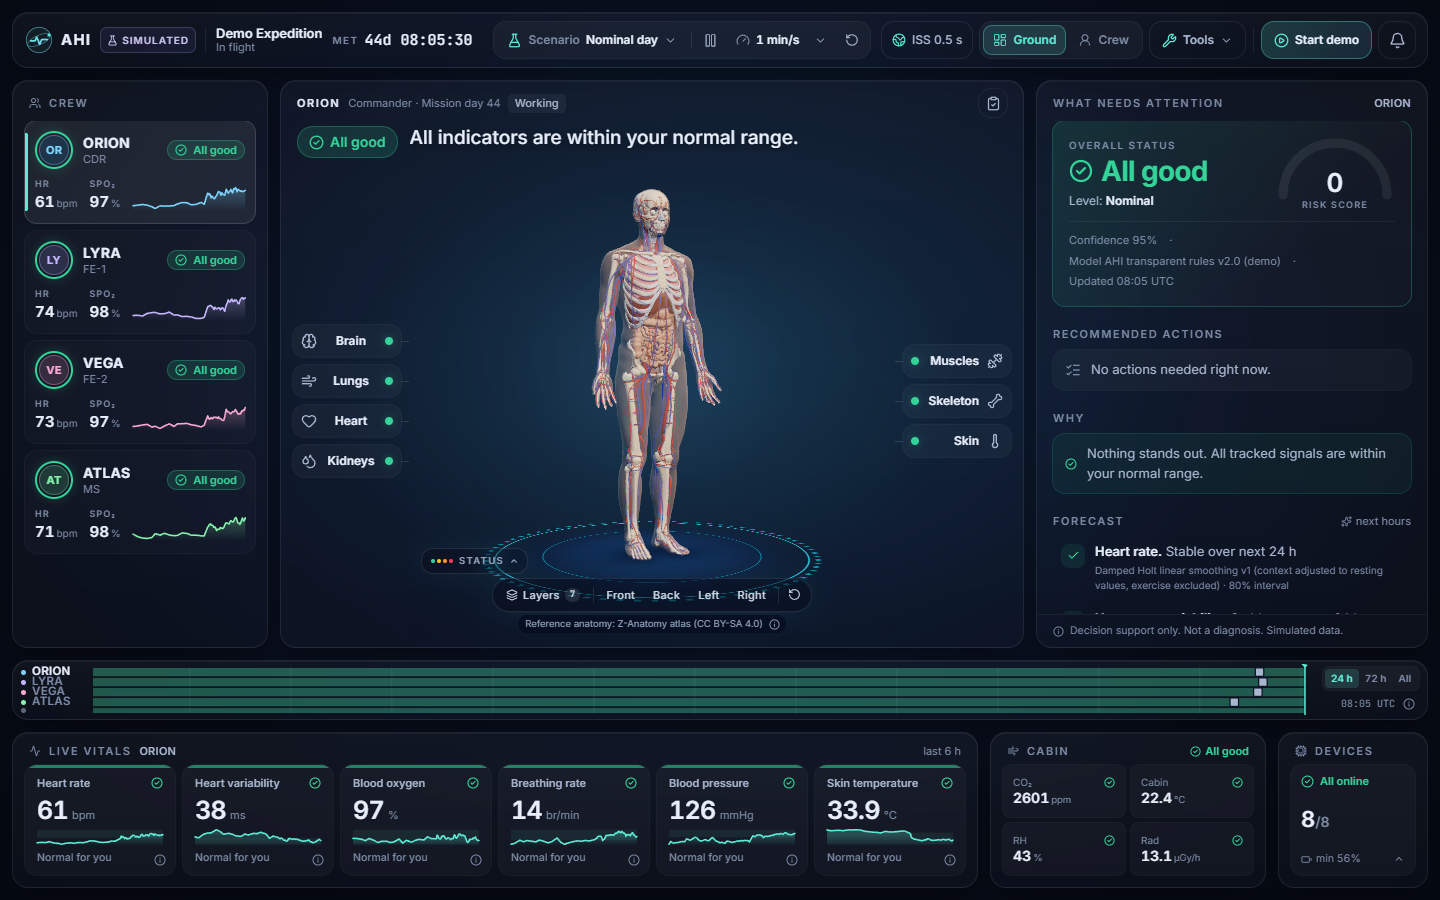
\includegraphics[width=0.54\linewidth]{images/screens/ground-view.png}};
\begin{scope}[x={(img.south east)},y={(img.north west)}]
\node at (0.62,0.955) {\callout{1}};
\node at (0.10,0.60) {\callout{2}};
\node at (0.40,0.62) {\callout{3}};
\node at (0.86,0.60) {\callout{4}};
\node at (0.50,0.23) {\callout{5}};
\node at (0.30,0.12) {\callout{6}};
\end{scope}
\end{tikzpicture}
\captionof{figure}{Ground view on a nominal day, with its six areas numbered. Simulated data.}
\label{fig:ground-view}
\end{minipage}
\par\medskip

\begin{enumerate}
\item[\callout{1}] \textbf{Top bar:} \texttt{SIMULATED} badge, mission profile (Launch, ISS, Moon, Mars transit), mission time, \textbf{scenario player} (scenario, play, speed, restart), \textbf{Earth link}, \textbf{Ground / Crew} toggle, \textbf{Tools}, \textbf{Start demo} and the \textbf{alerts bell}.
\item[\callout{2}] \textbf{Crew rail} (left): one card per astronaut (ORION, LYRA, VEGA, ATLAS) with status in plain words, heart rate, blood oxygen and a six hour sparkline. Click a card or press \key{1} to \key{4}; the rest of the screen follows.
\item[\callout{3}] \textbf{3D body} (center): body systems that need attention light up in their status color; the heart beats at the live heart rate and the lungs breathe at the live breathing rate. Body system chips sit beside it.
\item[\callout{4}] \textbf{What needs attention} (right): status, risk score, actions, reasons and forecast.
\item[\callout{5}] \textbf{Status timeline:} one lane per astronaut plus the cabin, with markers for alerts, actions, check-ins and messages.
\item[\callout{6}] \textbf{Live vitals, cabin and devices} (bottom): six vitals against the personal normal, cabin CO\textsubscript{2}, temperature, humidity and radiation, and the state of every device.
\end{enumerate}
